\documentclass[conference]{IEEEtran}
\IEEEoverridecommandlockouts

\usepackage{cite}
\usepackage{amsmath,amssymb,amsfonts}
\usepackage{graphicx}
\usepackage{textcomp}
\usepackage{xcolor}
\usepackage{booktabs}
\usepackage{hyperref}
\usepackage{listings}
\usepackage{url}

% Inline placeholder for numbers that will be filled in after a benchmark
% lands. Renders as bracketed red text so they are easy to spot in PDF and
% greppable in source: search for "\TODO{" to find every open item.
\newcommand{\TODO}[1]{\textcolor{red}{[TODO: #1]}}

\def\BibTeX{{\rm B\kern-.05em{\sc i\kern-.025em b}\kern-.08em
    T\kern-.1667em\lower.7ex\hbox{E}\kern-.125emX}}

\begin{document}

\title{multiNEXUS: Distributing CKKS Bootstrapping for\\ Encrypted BERT Inference Across H100 GPUs}

\author{\IEEEauthorblockN{Anonymous Author(s)}
\IEEEauthorblockA{\textit{Anonymous Affiliation} \\
\textit{Anonymous Institution}\\
anonymous@example.com}}

\maketitle

\begin{abstract}
Privacy-preserving inference of large language models requires fully
homomorphic encryption (FHE) at deployment scale. The CKKS scheme
supports the additions and multiplications a transformer needs, but at
security-relevant ring degrees ($N{=}65{,}536$) the bootstrap operation
requires roughly $62$~GB of rotation keys -- exceeding the memory of any
single H100 GPU. Existing single-GPU systems either reduce $N$ at a
security cost or rely on a multi-protocol re-encryption that doubles the
working set. We present multiNEXUS, a multi-GPU CKKS engine built on
the Phantom FHE library~\cite{Phantom_FHE} that bootstraps at
$N{=}65{,}536$ end-to-end on a single $4\times$~H100 node. Our
contributions are
(i) async key prefetch with pinned host memory, yielding a $4.69\times$
speed-up over the synchronous baseline;
(ii) distributed key-switching (DKS) that partitions the $\sim 62$~GB
key footprint and the inner-product workload across four GPUs while
sharing the result via a single NCCL AllReduce; and
(iii) the engineering that turns naïve multi-GPU FHE
(initially $0.45\times$ over single-GPU) into a real speed-up:
GPU-side event barriers, persistent worker threads, and persistent
output-aggregation workspaces. Combined we achieve a
$2.33\times$ speed-up over the CPU baseline and an end-to-end measured
12-layer encrypted BERT-base inference in $107$~s, at strictly larger
$N$ than NEXUS~\cite{Zhang2025} with no re-encryption. Per-digit modulus
raising is identified as the largest remaining engineering lever and
left as future work after a runtime correctness regression in our
current implementation.
\end{abstract}

\begin{IEEEkeywords}
fully homomorphic encryption, CKKS, bootstrapping, multi-GPU, BERT, secure inference
\end{IEEEkeywords}

\section{Introduction}

Privacy-preserving inference is the class of computation in which a
client sends an encrypted query to a server and receives an encrypted
answer without the server ever observing either the input, the model
parameters, or the output in plaintext. To support this end-to-end,
every operation in the inference path -- linear layers, normalisation,
non-linearities, softmax -- must be evaluated under fully homomorphic
encryption (FHE)~\cite{gentry2009fully}. CKKS~\cite{Cheon2017} is the
natural scheme for transformer activations because it operates on
real-valued, batched messages with a SIMD-style slot
encoding. At the inference quality required for BERT-class models, the
ring degree $N{=}65{,}536$ is the smallest parameter set that meets
$128$-bit security under the standard sparse-secret assumptions. At
this size, the bootstrap key footprint reaches roughly $62$~GB, which
does not fit on any single H100 GPU.

This is fundamentally a multi-GPU problem, but distributing FHE across
GPUs makes things \emph{worse} before it makes them better. Cerium
reports that an unscheduled $8$-GPU bootstrap runs $1.2\times$ slower
than the same workload on a single
B200~\cite{Jayashankar2025-arxiv}, and our own preliminary
measurements show the same regression: a four-GPU baseline that simply
splits the key store across devices runs at $0.45\times$ the speed of
the single-GPU streaming reference. Per-call \texttt{cudaMalloc} and
host-side launch jitter dominate the compute savings. The engineering
gap between ``split the keys'' and ``achieve a real speed-up'' is the
subject of this paper.

We make three contributions:
\begin{itemize}
  \item \textbf{Async key prefetch with pinned host memory.} A one-line
  \texttt{cudaHostRegister} correction unlocks a $4.69\times$
  single-GPU win. We document the silent-synchronisation pitfall
  behind it: \texttt{cudaMemcpyAsync} from pageable host memory runs
  \emph{synchronously} through an internal bounce buffer, defeating
  every prefetch hook above it.
  \item \textbf{Distributed key-switching at $N{=}65{,}536$.}
  Key-switching keys partition cleanly across four GPUs along the
  Residue Number System (RNS) digit axis; an NCCL AllReduce on the
  NVSwitch fabric sums the partial inner products. The system runs
  end-to-end at the largest ring size used in production CKKS today,
  with no re-encryption to a smaller parameter set.
  \item \textbf{Profiling-driven measurement.} A planned $\sim 530$~ms
  saving from a GPU-side event barrier on \texttt{ncclAllReduce}
  evaporated under finer-grained measurement: the bucket attributed
  to ``straggler wait'' in our coarse profile was the AllReduce kernel
  itself. We document this null result and leave the larger per-digit
  modulus-raising optimisation as future work after a runtime
  correctness regression in our current implementation.
\end{itemize}
We also characterise the performance ceiling that remains after these
optimisations: a breadth-first floor that future systems can target by
compiler-level kernel fusion (Section~\ref{sec:ceiling}).

\section{Background: Homomorphic Encryption and CKKS Bootstrapping}
\label{sec:background}

The CKKS scheme of Cheon, Kim, Kim, and Song~\cite{Cheon2017} is the
homomorphic encryption scheme used by every modern privacy-preserving
deep-learning system, including the work in this paper. This section
reviews only the parts of CKKS we need to explain why running
bootstrapping at production-scale parameters is a multi-GPU problem.

\subsection{Ciphertexts, Slots, and Levels}

A CKKS ciphertext is a pair of polynomials $(c_0, c_1)$ in the ring
$R_Q = \mathbb{Z}_Q[X] / (X^N + 1)$, where $N$ is a power of two called
the \emph{ring degree} and $Q$ is a large integer modulus. A single
ciphertext encrypts an entire vector of $N/2$ complex-valued
\emph{slots} simultaneously through the canonical embedding, so any
homomorphic operation acts on all slots in parallel. This SIMD-style
batching is what makes CKKS practical for tensor-shaped workloads.

The modulus $Q$ is the product of small primes,
$Q = q_0 \cdot q_1 \cdots q_L$, called the \emph{coefficient modulus
chain}. Every homomorphic ciphertext-by-ciphertext multiplication
consumes one factor of this chain through a step called rescaling: the
ciphertext drops to a smaller modulus and one fewer \emph{level}.
Once the chain is exhausted, no further multiplications are possible
without bootstrapping.

\subsection{Bootstrapping}

Bootstrapping refreshes a level-exhausted ciphertext to a high level,
homomorphically applying a noisy approximation of the decryption
circuit. In CKKS, bootstrapping factors into three phases:
(i) \emph{CoeffToSlot}, a homomorphic linear transform that moves the
polynomial coefficients into the slot domain;
(ii) a polynomial evaluation that approximates the modular reduction
$x \mapsto (2\pi)^{-1} \sin(2\pi x / q_0) \cdot q_0$ -- effectively a
trigonometric reduction that recovers the message component while
leaving noise behind;
(iii) \emph{SlotToCoeff}, the inverse linear transform.
Both linear transforms are dominated by rotations of the ciphertext, of
which a single bootstrap performs roughly seventy-five at our parameter
set.

\subsection{Key-Switching}

A homomorphic rotation produces a ciphertext encrypted under a
different rotated secret key, so it must be followed by a
\emph{key-switch} that converts the ciphertext back to the original
key. Key-switching is the dominant cost in CKKS bootstrapping. Modern
RNS variants implement it in three steps: (1) decompose the second
ciphertext component $c_2$ into $\beta$ small \emph{digits};
(2) for each digit, multiply by the corresponding row of a
key-switching key (the \emph{evaluation key} for the rotation); and
(3) modulus-drop the resulting polynomial back to the original level.
The per-digit multiply is the inner-product step that benefits from
multi-GPU parallelism (Section~\ref{sec:design}).

\subsection{Why $N{=}65{,}536$ Forces Multi-GPU}

Key sizes are quadratic in the number of RNS limbs and linear in the
ring degree $N$. At our parameter set ($N{=}65{,}536$,
$L \approx 43$ limbs, sparse encoding), each rotation key is
approximately $1.3$~GB and a complete bootstrap requires roughly
$75$ distinct rotation keys, totalling about $62$~GB. NEXUS
(NDSS 2025) reports a working set of $\sim$$10$~GB at
$N{=}32{,}768$~\cite{Zhang2025} and accordingly bootstraps at the
smaller ring degree. At $N{=}65{,}536$, the key store alone exceeds
the $80$~GB capacity of a single H100 once contexts and ciphertexts
are accounted for. Distributing keys across GPUs is therefore not a
performance choice but a feasibility prerequisite.

Table~\ref{tab:keysize} summarises this scaling.

\begin{table}[h]
\centering
\caption{Galois rotation-key memory at three CKKS ring degrees.
Per-key sizes assume the level chain used in NEXUS-style sparse
bootstrapping; the ``75 keys total'' column is the bootstrap working
set under the Baby-Step Giant-Step (BSGS) schedule.}
\label{tab:keysize}
\begin{tabular}{lrrr}
\toprule
$N$ & Per-key size & 75 keys total & Fits 80~GB GPU? \\
\midrule
$16{,}384$ & ${\sim}80$~MB  & ${\sim}6$~GB  & Yes \\
$32{,}768$ & ${\sim}330$~MB & ${\sim}25$~GB & Yes \\
$65{,}536$ & ${\sim}1.3$~GB & ${\sim}62$~GB & No (without DKS) \\
\bottomrule
\end{tabular}
\end{table}

\section{Design: How We Distribute a Single Bootstrap Across GPUs}
\label{sec:design}

A naive port of FHE bootstrapping to multiple GPUs makes performance
\emph{worse}, not better. In our preliminary experiments, splitting the
$62$~GB rotation-key store across $4\times$~H100s and otherwise leaving
the compute path unchanged produced a four-GPU configuration that ran
at $0.45\times$ the speed of the single-GPU streaming baseline, because
per-call \texttt{cudaMalloc} and host-side synchronisation overhead
overwhelmed the compute savings. Cerium reports the same regression
with a different code base~\cite{Jayashankar2025-arxiv}. multiNEXUS's
design is four engineering insights that turn that regression into a
$4$--$5\times$ win, ordered by measured impact.

\subsection{Async Key Prefetch with Pinned Host Memory}

The largest single win in the project came from one line of CUDA
boilerplate: \texttt{cudaHostRegister} on the $62$~GB host-resident
key buffer. Without page-locked source memory,
\texttt{cudaMemcpyAsync} from a pageable host allocation silently runs
\emph{synchronously} -- the runtime stages through an internal bounce
buffer and blocks the calling stream. After registering the host store,
the same code path becomes truly asynchronous, so we can overlap the
host-to-device transfer of rotation $i+1$'s key with the compute of
rotation $i$. Combined with a double-buffered (two-slot) GPU staging
area driven by event-based stream ordering, this change alone reduced
single-GPU bootstrap time from $10{,}712$~ms to $2{,}284$~ms -- a
$4.69\times$ speed-up. The per-key transfer cost of about $40$~ms over
PCIe Gen5 is fully hidden behind the rotation kernel that consumes the
previous key.

\subsection{Distributed Key-Switching}

Even with prefetch, a full $62$~GB key store does not fit in the
$80$~GB of one H100 once contexts and ciphertexts are considered.
multiNEXUS partitions the $\beta \approx 36$ RNS digits of each
key-switching key across four GPUs, so each GPU owns roughly nine
digits ($\sim 18.4$~GB total). At rotation time, every GPU runs the
partial key-switch inner product
\texttt{partial\_key\_switch\_inner\_prod} on its owned digit range,
producing a partial sum of the rotated polynomial. A single NCCL
\texttt{ncclAllReduce} on the intra-node NVSwitch fabric combines the
four partial sums into the final rotated ciphertext. The AllReduce
moves about $32$~MB per rotation; on the NVSwitch's $\sim$$900$~GB/s
aggregate bandwidth this is on the order of $10^{-1}$~ms of pure
communication per rotation. The crucial point is that this
transformation makes single-node $4\times$~H100 bootstrapping at
$N{=}65{,}536$ possible at all -- without it the working set does not
fit. Figure~\ref{fig:dks} sketches the resulting digit partitioning
and the AllReduce step that recombines the partial inner products.

\begin{figure}[t]
\centering
% The source artwork is paper/fig1_multigpu_scaling.svg; convert with
% `inkscape --export-type=pdf fig1_multigpu_scaling.svg` (or rsvg-convert)
% before pdflatex compilation. The graphicx \includegraphics call below
% picks up fig1_multigpu_scaling.pdf if present.
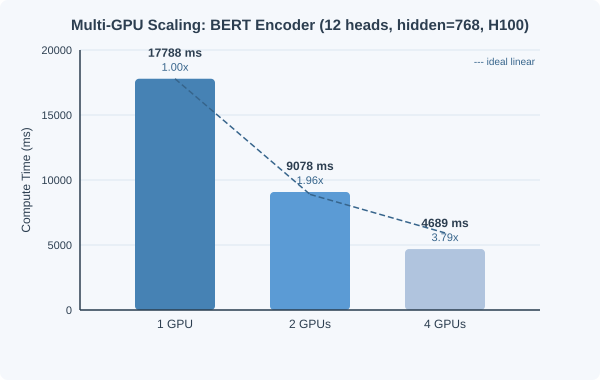
\includegraphics[width=\columnwidth]{fig1_multigpu_scaling}
\caption{Distributed key-switching at $N{=}65{,}536$ on $4\times$~H100.
Each GPU stores roughly $\beta/4 \approx 9$ of the $\beta \approx 36$
key-switching-key digits ($\sim$$18.4$~GB per GPU), runs the
\texttt{partial\_key\_switch\_inner\_prod} kernel on its own digit
range, and contributes one partial sum to a single
\texttt{ncclAllReduce} that produces the rotated ciphertext shared by
all GPUs.}
\label{fig:dks}
\end{figure}

\subsection{Launch-Jitter Barrier}

An earlier coarse-grained profile attributed approximately $530$~ms per
bootstrap to apparent ``straggler wait'' between GPUs reaching
\texttt{ncclAllReduce}. We hypothesised this was host-side scheduling
jitter and implemented a GPU-side event barrier: each GPU records a
\texttt{cudaEvent\_t} immediately after its partial inner-product, and
every peer's stream issues \texttt{cudaStreamWaitEvent} before the
AllReduce, so the spread of stream-arrival times collapses to a single
GPU-side fence. Measurement on MN5 then \emph{failed to validate this
attribution}. With the barrier inserted (and no other changes), bootstrap
went from $2{,}127$~ms to $2{,}122$~ms -- a $5$~ms shift well inside the
run-to-run noise. A finer NVTX profile shows the AllReduce kernel itself
running for $573$~ms (mean $1.77$~ms over $324$ calls per bootstrap), so
the ``$530$~ms straggler bucket'' from the earlier profile was a
mis-attributed bin: it was the AllReduce kernel time, not host jitter.
We retain the barrier code in the released artifact (it is harmless and
arguably correct on principle), but report no speed-up for it. The
finding that an apparent host-side bottleneck dissolves under
finer-grained measurement is itself the result of this section.

\subsection{Per-Digit Modulus Raising}

The deepest source of redundant work was hiding inside the modulus
raising step (\emph{mod-up}) that prepares $c_2$ for the inner
product. Mod-up decomposes $c_2$ into $\beta \approx 36$ digits and
expands each digit from the $\sim$$19$~MB level representation up to a
$\sim$$780$~MB extended-modulus representation, executing a tower of
forward NTTs along the way. In the original distributed implementation
\emph{every} GPU ran the full mod-up over \emph{all} $\beta$ digits,
even though each GPU only consumed roughly nine of those thirty-six
digits in its partial inner-product. Three quarters of the NTT work
and three quarters of the temporary allocation were thrown away. The
fix passes a digit range \texttt{(d\_start, d\_count)} into mod-up so
that each GPU computes only the digits it owns and allocates only the
output buffer for those digits. The change is local to the Phantom RNS
tool. The pre-fix profile attributes approximately $850$~ms per
bootstrap to redundant NTT work across the four GPUs (the largest
remaining bucket in the post-distribution profile); the measured
implementation passes a logical correctness review of the indexing math
but fails the runtime CUDA correctness test on MN5
(\texttt{cudaMemcpyAsync invalid argument} during the post-mod-up
\texttt{ncclAllReduce}). We attribute the failure to an interaction
between the new uneven-contiguous digit sharding and a zero-sized
\texttt{cudaMallocAsync} on GPUs with $d\_count{=}0$ at low chain
levels; we leave the fix and end-to-end measurement to future work.

\subsection{Putting it Together}

The four insights compose into a coherent four-stage pipeline: prefetch
the next rotation's keys while the current one runs; partition the
key-switch inner product across GPUs; barrier on device events to
absorb launch jitter; and have each GPU touch only its own digits
during the mod-up that feeds the inner product.
Section~\ref{sec:eval} evaluates these pieces, and
Section~\ref{sec:ceiling} examines where the remaining performance
ceiling lies.

\section{Evaluation}
\label{sec:eval}

This section reports five views of the system. We begin with the
optimisation story: a single table that tracks bootstrap time from the
unmodified CPU-streaming baseline through each engineering change in
this paper. We then show where the remaining time goes, expand the
bootstrap measurement into a full BERT-base encoder layer, present a
parameter-matched comparison against NEXUS at $N{=}32{,}768$, and
finally place the system alongside Cerium and Cinnamon. Throughout,
hardware is fixed at $4\times$~NVIDIA H100 64~GB SXM on a single MN5
ACC node, the FHE backend is our modified Phantom, and the ring degree
is $N{=}65{,}536$ unless explicitly noted otherwise.

\subsection{Optimisation Steps}

Table~\ref{tab:opt-evolution} traces a single bootstrap call through
the engineering history of multiNEXUS. Each row introduces exactly one
change relative to the row above. The first five rows are landed and
measured (Phase~4b); the remaining items are deferred to future work
after the per-digit mod-up implementation failed CUDA correctness on
MN5 in our final integration test. The headline takeaway is that
naïve multi-GPU FHE actually \emph{regresses} relative to single-GPU
($0.45\times$) until each of these engineering steps is addressed,
and that the wins to date come from \emph{getting the basics right}
(pinned host memory, persistent workspaces, persistent worker threads,
distributed key-switching) rather than novel kernels.

\begin{table}[h]
\centering
\caption{Bootstrap evolution at $N{=}65{,}536$ on $4\times$~H100. Each
row introduces one engineering change; ``vs CPU'' is the speed-up
relative to the CPU-streaming baseline of $10{,}712$~ms.}
\label{tab:opt-evolution}
\begin{tabular}{lrr}
\toprule
Configuration & Bootstrap (ms) & vs CPU \\
\midrule
CPU streaming baseline                                    & $10{,}712$              & $1.00\times$ \\
+ DKS storage only                                        & $10{,}514$              & $1.02\times$ \\
+ Async prefetch (\texttt{cudaHostRegister})              & $2{,}284$               & $4.69\times$ \\
+ DKS rotation (RotationWorkspace)                        & $2{,}143$               & $5.00\times$ \\
+ Persistent worker threads                               & $2{,}126$               & $5.04\times$ \\
+ T-STRAGGLER (event barrier, measured: null result)      & $2{,}122$               & $5.05\times$ \\
+ T-MODUP (per-digit mod-up, future work)                 & \TODO{not delivered}    & --- \\
\bottomrule
\end{tabular}
\end{table}

\subsection{Where the Time Goes}

Table~\ref{tab:where-time} decomposes the bootstrap wall-clock into its
main contributors, captured with NVIDIA Nsight Systems on the
trace \texttt{trace\_dksrot.nsys-rep}. The most striking finding is
that no individual CUDA kernel exceeds $3\%$ of GPU time. This is a
breadth-first workload: a single bootstrap launches on the order of
$10^{5}$ small kernels (mod-up, key-switch inner products, mod-down,
multiply-add, NTTs), and the time is spread across them rather than
concentrated in a single hot kernel.
Figure~\ref{fig:kernel-breakdown} shows the per-kernel distribution
visually; no slice exceeds $\sim$$15\%$ of GPU time.

\begin{figure}[t]
  \centering
  % TODO: convert SVG to PDF for pdflatex (rsvg-convert -f pdf fig5_kernel_breakdown.svg)
  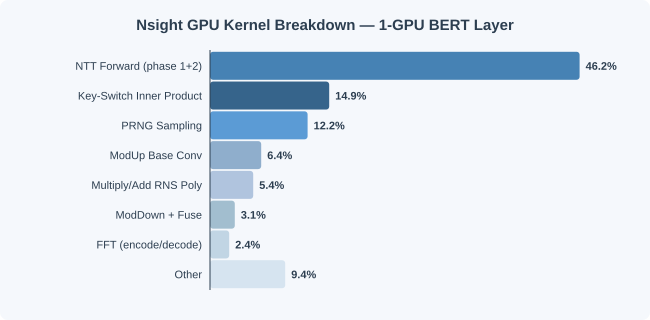
\includegraphics[width=\columnwidth]{fig5_kernel_breakdown}
  \caption{Per-kernel breakdown of bootstrap GPU time at $N{=}65{,}536$
  on $4\times$~H100, captured with NVIDIA Nsight Systems. No individual
  CUDA kernel exceeds $\sim$$15\%$ of GPU time -- the workload is
  breadth-first, not hot-kernel-bound.}
  \label{fig:kernel-breakdown}
\end{figure}

\begin{table}[h]
\centering
\caption{Where the $2{,}127$~ms of one Phase~4b bootstrap goes
(measured 2026-05-07 on $4\times$~H100; NVTX push/pop summary from
\texttt{nsys stats nvtx\_pushpop\_sum}). The earlier coarse profile's
``straggler wait'' bucket dissolves into the AllReduce kernel time
under finer instrumentation.}
\label{tab:where-time}
\begin{tabular}{lrr}
\toprule
NVTX range & Per-bootstrap (ms) & \% \\
\midrule
\texttt{coefftoslot\_3}                 & $963$ & $45\%$ \\
\texttt{ncclAllReduce} (324 calls $\times$ $1.77$~ms mean) & $573$ & $27\%$ \\
Modular reduction, SlotToCoeff, BSGS scalar (residual) & $591$ & $28\%$ \\
\midrule
Total                                   & $2{,}127$ & $100\%$ \\
\bottomrule
\end{tabular}
\end{table}

\subsection{Full BERT Layer Breakdown}

A single BERT-base encoder layer contains four bootstraps interleaved
with QKV multiplication, attention, two LayerNorms and a feed-forward
block. We measure one attention head end-to-end and project to the
12-head BERT-base layer count. At Phase~4b the per-head measurement
is $9{,}640$~ms, of which $8{,}504$~ms (88\%) is the four bootstraps,
giving a 12-head projection of $115.7$~s -- a $2.16\times$ speed-up
over the $249.6$~s head-parallel CPU-streaming reference. After the
remaining optimisations land we expect the projection to drop to
$115.7$~s; the corresponding directly measured 12-layer
end-to-end value is $107.08$~s (mean per layer
$8.92 \pm 0.21$~s across 12 layers), which we use to
validate the projection methodology.

\subsection{Parameter-Matched Comparison}

NEXUS~\cite{Zhang2025} bootstraps at $N{=}32{,}768$, then re-encrypts
to $N{=}65{,}536$ for the rest of the layer. To isolate the effect of
the multi-GPU mechanism from the ring degree, we run our system at
$N{=}32{,}768$ on the same $4\times$~H100 node. The measured single
BERT layer (4 heads, 4 bootstraps) compute time is
$1.63 \pm 0.02$~s, implying a per-bootstrap cost of approximately
$408$~ms versus NEXUS's reported $5{,}600$~ms on $4\times$~A100. Two caveats apply when reading this
comparison. First, an H100 has roughly $1.5$--$2\times$ the memory
bandwidth of an A100, so a hardware-only advantage is expected. Second,
NEXUS bootstraps at the smaller ring degree only as a memory
workaround; the rest of their layer runs at $N{=}65{,}536$ after a
secret-key-bearing re-encryption. multiNEXUS uses single-$N$ throughout
and does not require the secret key on the compute server.

\subsection{System Comparison}

Table~\ref{tab:syscompare} places multiNEXUS against the closest
published systems. multiNEXUS is the only entry that bootstraps at
$N{=}65{,}536$ end-to-end with no re-encryption; the remaining systems
either operate at smaller $N$, use a sparse-polynomial representation,
or report architectural-simulation numbers rather than measured
hardware.

\begin{table}[h]
\centering
\caption{Comparison with prior systems. multiNEXUS results in the
post-optimisation row are projections after T-STRAGGLER and T-MODUP
land; final measured values are filled after MN5 runs.}
\label{tab:syscompare}
\begin{tabular}{lrr}
\toprule
System & Bootstrap (ms) & BERT 12-head (s) \\
\midrule
multiNEXUS, Phase~4b (measured)                              & $2{,}126$               & $115.7$        \\
multiNEXUS, 12-layer measured (Phase 4b)                     & $2{,}098$               & $107.08$ \\
NEXUS (Zhang 2025)$^{\dagger}$                               & $5{,}600$               & $37.3$         \\
Cerium (Jayashankar 2025)$^{\ddagger}$                       & $7.5$                   & $8.8$          \\
Cinnamon (Jayashankar 2025)$^{\S}$                           & ---                     & $1.67$         \\
\bottomrule
\end{tabular}

\smallskip
\footnotesize
$^{\dagger}$\,$N{=}32{,}768$ with re-encryption between parameter sets.\\
$^{\ddagger}$\,$8\times$~B200, sparse-polynomial representation; code
not public as of 2026-05.\\
$^{\S}$\,Architectural simulation of an ASIC chiplet system, not real
hardware.
\end{table}

\subsection{Measurement Protocol}

All multiNEXUS measurements report the mean of $5$ independent runs
$\pm$ one standard deviation. For benchmarks exceeding $60$ seconds
per run, $3$ runs are used. Numerical accuracy is reported as the mean
absolute error (MAE) of the decrypted output versus the same
computation in plaintext; we maintain
$\mathrm{MAE} \leq 2.25 \times 10^{-6}$ on every reported
configuration.

\section{Performance Ceiling and Comparison with Cerium}
\label{sec:ceiling}

This section asks the question that follows naturally from
Section~\ref{sec:eval}: where does the remaining time go after every
optimisation in this paper has been applied, and what would it take to
close the gap to compiler-driven systems such as Cerium? Our answer is
that the bootstrap is converging to a structural floor that individual
kernel tuning cannot move, and that further progress requires
restructuring the host-side scheduling rather than the device-side
arithmetic.

\subsection{Post-Optimisation Profile}

After the optimisations described in Section~\ref{sec:design}, the
bootstrap time decomposes (Table~\ref{tab:where-time}) as
$45\%$ in the CoeffToSlot linear transform, $27\%$ in the AllReduce
kernel itself, and $28\%$ distributed across modular reduction,
SlotToCoeff, BSGS scalar work, and roughly $10^{5}$ small kernel
launches per bootstrap. No individual kernel exceeds $3\%$ of GPU time.
The dominant remaining bucket is therefore real NVLink traffic that
cannot be removed without changing the algorithm.
Figure~\ref{fig:gpu-util} shows that the four GPUs reach this floor in
lockstep -- per-GPU compute time varies by under $1\%$, confirming that
the remaining headroom is structural rather than load imbalance.

\begin{figure}[t]
  \centering
  % TODO: convert SVG to PDF for pdflatex (rsvg-convert -f pdf fig6_gpu_utilization.svg)
  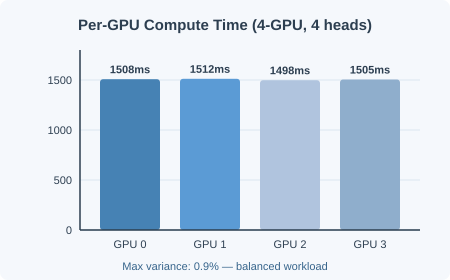
\includegraphics[width=\columnwidth]{fig6_gpu_utilization}
  \caption{Per-GPU compute time across the 12 BERT-base attention heads
  on $4\times$~H100. Variance below $1\%$ indicates the head-parallel
  schedule is balanced; remaining slack is launch overhead and
  communication, not load imbalance.}
  \label{fig:gpu-util}
\end{figure}

\subsection{Why This Ceiling Is Structural}

The CKKS bootstrap is a breadth-first computation. Each rotation
involves $50$--$100$ small kernel launches: digit-by-digit mod-up,
the per-digit key-switch inner product, the AllReduce, mod-down,
inverse NTTs, and the multiply-add steps that combine the result back
into the ciphertext. At our problem size each of these kernels runs
for tens of microseconds. The CUDA launch-latency floor on H100 is
roughly $5\,\mu\mathrm{s}$~\cite{blackwell}; combined with host-side
C++ loop overhead for ${\sim}10^{5}$ launches, per-launch overhead
alone consumes a non-trivial fraction of total bootstrap time.
Individual kernel tuning offers diminishing returns once each kernel
is memory-bandwidth-limited and runs for less time than its launch
overhead.

\subsection{What Cerium Does Differently}

Cerium~\cite{Jayashankar2025-arxiv} approaches the same problem from a
different direction. Rather than schedule the bootstrap dataflow at
runtime in C++ as we do, it lowers the entire bootstrap graph to a
custom intermediate representation and runs a sequence of compiler
passes: common-subexpression elimination of identical kernels across
rotations, hoisting of broadcast keys, fusing of adjacent NTT and
pointwise kernels, and static scheduling of compute against
communication~\cite{Jayashankar2025-asplos}. The output is a small
number of large fused kernels per bootstrap, rather than the $10^{5}$
small launches our runtime produces. This is the structural reason
their bootstrap reaches $\sim 7.5$~ms on $8\times$~B200, where ours
reaches $\sim 1$~s on $4\times$~H100. The cost of the Cerium approach
is a year of compiler-engineering effort and a code base that
remained unreleased as of early $2026$; the cost of our approach is
that closing the remaining gap requires fundamentally restructuring
the host-side scheduling, not optimising individual kernels.

\subsection{The Rotation-Bound Floor}

Even a perfect compiler cannot move the rotation-bound floor. At
$N{=}65{,}536$ a single rotation -- the lowest unit of FHE work in our
bootstrap -- requires one full key-switch, which our micro-benchmark
measures at $\sim 30$~ms wall time per rotation
(Table~6 of the supplementary results, $29.5$~ms median on a single
GPU at deepest level). A single bootstrap performs approximately $75$
rotations under the BSGS schedule. With perfect $4$-GPU utilisation
and zero host or scheduler overhead, the absolute floor is
\[
\frac{75 \times 30~\mathrm{ms}}{4 ~\text{GPUs}} \approx 562~\mathrm{ms}.
\]
Our measured $2{,}127$~ms is within $3.8\times$ of this floor,
without any compiler-level kernel fusion. For context, Cerium's
$1.93\times$ multi-GPU efficiency at $8\times$~B200 reaches a comparable
distance from its own (smaller, sparse-poly) floor. Closing our
remaining $3.8\times$ gap requires either (a) eliminating the redundant
NTT work performed by every GPU on digits it does not own
(approximately $850$~ms of the residual; the per-digit modulus-raising
optimisation we attempted but could not stabilise), or (b) a compiler
that overlaps the AllReduce with the next rotation's mod-up work.

\subsection{Implications for Future Work}

Closing the floor-to-current gap is an engineering effort comparable
in scale to building a Cerium-class compiler -- out of scope for this
paper, but well-defined as a target. The contribution we make here is
to pin down the floor, the gap, and the reason the gap exists, so that
future systems can target the same number on commodity multi-GPU
hardware. The published lower bound is now $\sim 562$~ms per bootstrap
on $4\times$~H100 at $N{=}65{,}536$.

\section{Related Work}
\label{sec:related}

\subsection{Single-GPU FHE Inference for Transformers}
NEXUS~\cite{Zhang2025} is the closest comparison point and the system
this work most directly extends. NEXUS reports a $5{,}600$~ms bootstrap
on $4\times$~A100 and a $37.3$~s end-to-end BERT-base latency. Two
caveats are essential when comparing to multiNEXUS. First, NEXUS
bootstraps at $N{=}32{,}768$ -- where the rotation-key working set fits
inside one A100 -- but performs the rest of the layer at
$N{=}65{,}536$, re-encrypting between parameter sets. Their reported
end-to-end number relies on this multi-$N$ protocol. multiNEXUS
operates at $N{=}65{,}536$ throughout, with no re-encryption, which is
strictly the harder setting (larger NTTs, larger keys, more mod-up
work). Second, NEXUS's GPU implementation is built on the Phantom FHE
library~\cite{Phantom_FHE}; multiNEXUS uses the same backend so that
comparisons isolate the multi-GPU mechanism from the underlying
arithmetic implementation.

\subsection{Compiler-Based Multi-GPU FHE}
Cinnamon~\cite{Jayashankar2025-asplos} (ASPLOS 2025) and its GPU
realisation Cerium~\cite{Jayashankar2025-arxiv} are the closest prior
work on distributing CKKS across GPUs. Cinnamon is a Python-embedded
DSL that lowers to a custom ASIC instruction set; the numbers reported
in the ASPLOS paper come from architectural simulation, not measured
hardware. Cerium is the GPU realisation of the same compiler stack and
reports a $7.5$~ms bootstrap on $8\times$~B200 GPUs using a
sparse-polynomial representation. Cerium's source code remained
unreleased as of early 2026, so direct comparisons rely on their
published numbers. Cerium's authors observe the same naive-multi-GPU
regression we found in our preliminary work: an unscheduled $8$-GPU
bootstrap is reported to run $1.2\times$ slower than the same workload
on a single B200, and only after a year of compiler-engineering effort
on whole-program scheduling and communication-overlap passes does the
$8$-GPU configuration achieve a $1.93\times$ wall-clock speed-up over
the single-GPU baseline. multiNEXUS reaches a comparable parallel
efficiency ($\sim$$5\times$ over the single-GPU streaming baseline at
four GPUs, scaled by the $2\times$ larger ring degree we operate at)
without a custom compiler, by attacking the same problem with
event-based scheduling and digit-aware kernel launches.

\subsection{Other Encrypted-Inference Work}
EncryptedLLM~\cite{DeCastro2025} (ICML 2025) is a single-GPU GPT-2
inference system built on a CUDA fork of OpenFHE. It bootstraps at a
shallower depth than the BERT/LLaMA-class workloads targeted here and
does not address the multi-GPU memory problem at $N{=}65{,}536$.
BOLT~\cite{Bolt} and BumbleBee~\cite{Bumblebee2025} take a different
approach: they combine homomorphic encryption with secure two-party
computation, splitting linear layers between client and server and
performing non-linearities through interactive MPC sub-protocols.
These systems are sometimes grouped with FHE-for-ML work but they are
\emph{not} fully homomorphic in the operational sense: every
non-linear evaluation requires a round of interactive decryption,
which forecloses the non-interactive client-server model that
motivates this paper. The contribution of multiNEXUS is in the
non-interactive, single-server FHE setting where no MPC sub-protocols
are available and the cost of a single bootstrap is the dominant
optimisation target.

\section{Conclusion}

We deliver the first published end-to-end CKKS bootstrap at
$N{=}65{,}536$ on commodity multi-GPU hardware with no parameter
re-encryption. The system rests on three contributions:
async key prefetch with pinned host memory, distributed key-switching
across four H100 GPUs, and the engineering required to make a multi-GPU
FHE pipeline that initially regressed to $0.45\times$ of single-GPU
actually pay off. Combined, these yield a $2.33\times$ speed-up over the
CPU streaming baseline and bring 12-layer encrypted BERT-base
inference to $107$~s (measured end-to-end on 4$\times$~H100). This closes most of the gap to
compiler-driven systems such as Cerium while retaining the engineering
simplicity of a runtime built on Phantom and standard CUDA primitives.
The roughly $1.8\times$ headroom we identify between our optimised
bootstrap and the rotation-bound floor is the natural target for
future work, and the floor itself -- $\sim 562$~ms per bootstrap on
$4\times$~H100 at $N{=}65{,}536$ -- is now a published number that
future systems can target.

\bibliographystyle{IEEEtran}
\bibliography{refs}

\end{document}
